% This file is part of the multi-tex ECE 486 Final Project Report 
% file name: report.tex

% YOU CAN COMPILE FROM THIS FILE, THIS IS THE MAIN FILE, read the following

% included files:
% (Makefile)
% Makefile -- run make Makefile (on Mac or Linux), it takes care of LaTeX compilation

% (*.PDF)
% report.pdf -- (this file) report file, print it out and submit it

% (*.TEX)
% report.tex -- main file, pdflatex this file (tested on Mac and Linux)
% 0-title-page.tex -- title page
% 1-introduction.tex -- chapter 1 
% 2-mathematical-model.tex -- chapter 1 (lagrange equations of motion) and chapter 4 (linearisation)
% 3-full-state-feedback-control-friction-compensation.tex -- chapter 2 and chapter 4 (two state and three state feedback controller design)
% 4-full-state-feedback-control-decoupled-observer.tex -- chapter 4 (controller design) and chapter 5 (observer design for estimated state)
% 5-conclusions.tex -- conclusion
% 6-extra-credit.tex -- (optional) add thsese pages if you have demoed chapter 6 and chapter 7

\documentclass[11pt,letterpaper,twoside]{article}
\usepackage{mathptmx} %Times font
\usepackage{graphicx}
\usepackage{amsmath}

% packages published by the American Mathematical Society
\usepackage{mathtools} % mathtools loads amsmath and adds some useful tools. See, http://tex.stackexchange.com/questions/43860/mathtools-vs-amsmath
\usepackage{amssymb}

% for the title page
\newcommand{\HRule}{\rule{\linewidth}{0.5mm}}

% my favorite font: charter
%\usepackage{charter}

% create hyper-links within the document
\usepackage{hyperref}

% for colored links
\usepackage{xcolor}
\definecolor{illinois_professional_blue}{cmyk}{60, 40, 5, 0}
\definecolor{illinois_professional_orange}{cmyk}{3, 55, 100, 0}
\definecolor{illinois_bold_blue}{cmyk}{100, 86, 24, 9}
\definecolor{illinois_bold_orange}{cmyk}{0, 62, 99, 0}

\hypersetup{colorlinks=true, linktoc=all, linkcolor=illinois_professional_blue,}

% adds bibliography to table of contents
% \usepackage[nottoc]{tocbibind}

% segregating bibliography and references
% \usepackage{multibib}
% \newcites{ltex}{References}

% every section starts on a new page
% redefining section
\let\stdsection\section\renewcommand\section{\newpage\stdsection} % Leslie Lamport warns it is better to create newcommand rather than overwrite existing command, especially LaTeX built-ins

\begin{document}
% line 1: no numbering for table of contents
\addtocontents{toc}{\protect\thispagestyle{empty}}

% This file is part of the multi-tex ECE 486 Final Project Report 
% file name: 0-title-page.tex

% YOU DO NOT COMPILE FROM THIS SINGLE FILE, read the following

% included files:
% (Makefile)
% Makefile -- run make Makefile (on Mac or Linux), it takes care of LaTeX compilation

% (*.PDF)
% report.pdf -- report file, print it out and submit it

% (*.TEX)
% report.tex -- main file, pdflatex this file (tested on Mac and Linux)
% 0-title-page.tex -- (this file) title page
% 1-introduction.tex -- chapter 1 
% 2-mathematical-model.tex -- chapter 1 (lagrange equations of motion) and chapter 4 (linearisation)
% 3-full-state-feedback-control-friction-compensation.tex -- chapter 2 and chapter 4 (two state and three state feedback controller design)
% 4-full-state-feedback-control-decoupled-observer.tex -- chapter 4 (controller design) and chapter 5 (observer design for estimated state)
% 5-conclusions.tex -- conclusion
% 6-extra-credit.tex -- (optional) add thsese pages if you have demoed chapter 6 and chapter 7
 
\begin{titlepage}
	\begin{center}

		\textsc{\LARGE University of Illinois at Urbana-Champaign}\\[1.5cm]

		% Title
		\HRule\\[0.4cm]
		{\huge \bfseries ECE 486 : Final Project Report \\[0.4cm] }
		\uppercase{Spring 2015}\\[0.5cm]

		\HRule\\[1.5cm]
                
                % Add your info and your lab partner's info. Also include your section and TA's name
		\noindent
		\begin{minipage}{0.4\textwidth}
			\begin{flushleft} \large
				\textbf{Benjamin Kuo} % can we remove the names of students? just insert a name like FirstName1 LastName1 for lab partner?
			\end{flushleft}
		\end{minipage}%
		\begin{minipage}{0.4\textwidth}
			\begin{flushright} \large
				\textbf{Zhichun Wan} % FirstName2 LastName2
			\end{flushright}
		\end{minipage}
		\\~\\
		\textit{Teaching Assistant}: Y\"{u}n Han\\ % change it to TA's Name?
		\textit{Day of Laboratory Section}: Tuesday 11:00-1:50 % also this line depends

		\vfill

		% Bottom of the page
		{\large \today} % you can explicitly use a date if you don't like \today

	\end{center}
\end{titlepage}










\tableofcontents

% line 2: no numbering for table of contents
\setcounter{page}{0}
% This file is part of the multi-tex ECE 486 Final Project Report 
% file name: 1-introduction.tex

% YOU DO NOT COMPILE FROM THIS SINGLE FILE, read the following

% included files:
% (Makefile)
% Makefile -- run make Makefile (on Mac or Linux), it takes care of LaTeX compilation

% (*.PDF)
% report.pdf -- report file, print it out and submit it

% (*.TEX)
% report.tex -- main file, pdflatex this file (tested on Mac and Linux)
% 0-title-page.tex -- title page
% 1-introduction.tex -- (this file) chapter 1 
% 2-mathematical-model.tex -- chapter 1 (lagrange equations of motion) and chapter 4 (linearisation)
% 3-full-state-feedback-control-friction-compensation.tex -- chapter 2 and chapter 4 (two state and three state feedback controller design)
% 4-full-state-feedback-control-decoupled-observer.tex -- chapter 4 (controller design) and chapter 5 (observer design for estimated state)
% 5-conclusions.tex -- conclusion
% 6-extra-credit.tex -- (optional) add thsese pages if you have demoed chapter 6 and chapter 7

\section{Introduction}
The goal of the final project was to design and compare different controllers for stabilizing the reaction wheel pendulum (RWP) at equilibrium positions. We first derived mathematical equations to model the system and then obtain parameters for the pendulum and rotor. Later we used two state-space approaches -- full state feedback and observer feedback to implement the controllers for stabilizing the pendulum. In addition, our group also implemented the two extra-credit sections.
\subsection{Sensors}
The RWP has two optical encoders for measuring the state of the system. One sensor measures the relative angular displacement of the pendulum and the base mount $\varphi_p$. The other sensor measures the angular displacement of the rotor relative to the pendulum $\varphi_r$. In our mathematical modelss, however, we used angular positions relative to the vertical axis normal to the ground. Therefore the angular positions we used were as follows:
$$\theta_p = \varphi_p$$
$$\theta_r = \varphi_p+\varphi_r$$
From this point forward, we will use subscript $r$ and $p$ to refer to the rotor relative to the pendulum and the pendulum and the base mount respectively.
\subsection{Actuators}
The RWP has one actuator which is a 24-Volt, permanent magnet DC motor that could produce a torque on the reaction wheel. According Newton’s third law, there will be a reaction torque on the motor and hence the pendulum. The reaction torque can be used to control the motion of the pendulum.
\subsection{Equilibrium Positions}
There are two equilibrium positions for the RWP. They are the up and down equilibrium point. The up equilibrium point is an unstable configuration. The pendulum will easily fall down without control when disturbance is applied. The down equilibrium point is a stable configuration as the pendulum will eventually return to this point even without control.
\subsection{Implementation}
In this lab, we used Matlab to design the controllers for the RWP. We used the built-in Simulink interface in Matlab to design the controllers graphically.
% This file is part of the multi-tex ECE 486 Final Project Report 
% file name: 2-mathematical-model.tex

% YOU DO NOT COMPILE FROM THIS SINGLE FILE, read the following

% included files:
% (Makefile)
% Makefile -- run make Makefile (on Mac or Linux), it takes care of LaTeX compilation

% (*.PDF)
% report.pdf -- report file, print it out and submit it

% (*.TEX)
% report.tex -- main file, pdflatex this file (tested on Mac and Linux)
% 0-title-page.tex -- title page 
% 1-introduction.tex -- chapter 1 
% 2-mathematical-model.tex -- (this file) chapter 1 (lagrange equations of motion) and chapter 4 (linearisation)
% 3-full-state-feedback-control-friction-compensation.tex -- chapter 2 and chapter 4 (two state and three state feedback controller design)
% 4-full-state-feedback-control-decoupled-observer.tex -- chapter 4 (controller design) and chapter 5 (observer design for estimated state)
% 5-conclusions.tex -- conclusion
% 6-extra-credit.tex -- (optional) add thsese pages if you have demoed chapter 6 and chapter 7

\section{Mathematical Model}
We first used the Lagrange's equations to get the differential equations describing the system and then linearize the equations around the equilibrium point at $\theta_p=\pi$.
\subsection{Derivation of differential equations from Lagrangian}
In order to use the Lagrange's equations we must first obtain the energy equations of our system. We will use the following nomenclature:\\
$KE$ kinetic energy\\
$PE$ potential energy\\
$J$ moment of inertia with respect to $\theta_p$\\
$J_r$ moment of inertia with respect to the rotor about its center of mass\\
$l$ distance from pivot to center of mass of pendulum and rotor\\
$k$ torque constant of motor\\
$i$ input current to motor\\
The equations are as follows:
$$KE_{\text{pendulum}} = \frac{1}{2}J\dot\theta_p^2$$
$$PE_{\text{pendulum}} = (l-l\cos(\theta_p))mg$$
$$KE_{\text{rotor}} = \frac{1}{2}J_r\dot\theta_p^2$$
$$PE_{\text{rotor}} = 0$$
The Lagrangians can then be derived from this as they are the difference between the kinetic energies form the potential energies.
$$L_{\text{pendulum}} = \frac{1}{2}J\dot\theta_p^2-(l-l\cos(\theta_p))mg$$
$$L_{\text{rotor}} = \frac{1}{2}J_r\dot\theta_p^2-0$$
Finally from where we can derive our Lagrange Equations by using this relationship:
$$\frac{d}{dt}\left(\frac{\partial L}{\partial\dot q_k}\right)-\frac{\partial L}{\partial q_k}=\tau_k, k = 1,...,n$$
(where $\tau$ is the generalized for ce or torque in this case) we can get our Lagrange equations, which are our differential equations:
$$\text{Lagrange Equation}_{\text{pendulum}} = J\ddot\theta_p+mgl\sin(\theta_p)=-ki$$
$$\text{Lagrange Equation}_{\text{rotor}} = J_r\ddot\theta_r=ki$$
We can rewrite this in a format we're more familiar with (noting that $\omega_{np}^2 = \frac{mgl}{J}$):
$$\ddot\theta_p+\omega_{np}^2\sin(\theta_p)=-\frac{k}{J}i$$
$$\ddot\theta_r=\frac{k}{J_r}i$$

Finally noting the lab manual we need to consider the fact that our input we provide to the system is not the current but rather a signal we denote as $u$. We must also consider a frictional force of the rotor which depends of the speed which we will denote as $F(\dot\theta_r)$. Finally to simplify our representation we will make the following substitutions: $a = \omega_{np}^2 = \frac{mgl}{J}$, $b_p = \frac{k_u}{J}$, and $b_r = \frac{k_u}{J_r}$

This results in the following equations:
$$\ddot\theta_p+a\sin(\theta_p)=-b_p(u+F(\dot\theta_r))$$
$$\ddot\theta_r=-b_r(u+F(\dot\theta_r))$$

\subsection{Linearization into State Space Form}

Based on what we learned we are going to provide linear control to stablize this system, and we know this is not a linear system. We must linearize this system and we linearized the equations at the equilibrium point $\theta_p=\pi$. We get the state-space equation of $\boldsymbol{\dot x = Ax+B}u$ in the form:

$$
\begin{bmatrix}
\delta\dot\theta_p\\
\ddot\theta_p\\
\delta\dot\theta_r\\
\ddot\theta_r
\end{bmatrix}
=
\begin{bmatrix}
0 & 1 & 0 & 0\\
a & 0 & 0 & 0\\
0 & 0 & 0 & 1\\
0 & 0 & 0 & 0
\end{bmatrix}
\begin{bmatrix}
\delta\theta_p\\
\dot\theta_p\\
\delta\theta_r\\
\dot\theta_r
\end{bmatrix}
+
\begin{bmatrix}
0\\
-b_p\\
0\\
b_r
\end{bmatrix}
u$$
where $\delta\theta_p = \theta_p-\pi$ and $\delta\theta_r = \theta_r$.\\

Since this matrix is not that interesting, we won't show all the mathematical steps of linearizing it, but the nonlinear element of interest is not hard to see that the derivitive of sine is cosine, and cosine of $\pi - \pi$ or $0$ is 1. Hence, the $a$ coefficient is all that remains in that term.

% This file is part of the multi-tex ECE 486 Final Project Report 
% file name: 3-full-state-feedback-control-friction-compensation.tex

% YOU DO NOT COMPILE FROM THIS SINGLE FILE, read the following

% included files:
% (Makefile)
% Makefile -- run make Makefile (on Mac or Linux), it takes care of LaTeX compilation

% (*.PDF)
% report.pdf -- report file, print it out and submit it

% (*.TEX)
% report.tex -- main file, pdflatex this file (tested on Mac and Linux)
% 0-title-page.tex -- title page 
% 1-introduction.tex -- chapter 1 
% 2-mathematical-model.tex -- chapter 1 (lagrange equations of motion) and chapter 4 (linearisation)
% 3-full-state-feedback-control-friction-compensation.tex -- (this file) chapter 2 and chapter 4 (two state and three state feedback controller design) 
% 4-full-state-feedback-control-decoupled-observer.tex -- chapter 4 (controller design) and chapter 5 (observer design for estimated state)
% 5-conclusions.tex -- conclusion
% 6-extra-credit.tex -- (optional) add thsese pages if you have demoed chapter 6 and chapter 7

\section{Full State Feedback Control with Friction Compensation}
Using the models we derived from above, we were then able to design the compensators to stabilize our system.
\subsection{Development of the PD Control with Friction Compensation}
We want to stabilize this system with a PD controller. Since this is a relatively big matrix we wanted to introduce some simplifications to it. We first reduced our system to a second order system using only the position for the pendulum and its derivative. This results in the following model:

$$
\begin{bmatrix}
\delta\dot\theta_p\\
\ddot\theta_p
\end{bmatrix}
=
\begin{bmatrix}
0 & 1\\
a & 0
\end{bmatrix}
\begin{bmatrix}
\delta\theta_p\\
\dot\theta_p
\end{bmatrix}
+
\begin{bmatrix}
0\\
-b_p
\end{bmatrix}
u$$

We then had to pick our desired poles for the closed loop system. We were given the requirements of having an $\omega_n > \omega_{np}$ and a $\zeta < \frac{1}{\sqrt{2}}$. We picked the following values: $\omega_n = 10$ and $\zeta = 0.5$. This resulted in these poles: $(3^\frac{1}{2}*5*j - 5)$,$(-3^\frac{1}{2}*5*i - 5)$.

From this we can use the MATLAB ``place'' function to generate the desired control matrix.

We also tried increasing the complexity and introduced the rotor speed into our control as well. In our three state feedback, we added an extra pole at -5, in between our previous poles and one at 0.

Like our two state control, our three state model is as follows:

$$
\begin{bmatrix}
\delta\dot\theta_p\\
\ddot\theta_p\\
\delta\dot\theta_r\\
\ddot\theta_r
\end{bmatrix}
=
\begin{bmatrix}
0 & 1 & 0 & 0\\
a & 0 & 0 & 0\\
0 & 0 & 0 & 1\\
0 & 0 & 0 & 0
\end{bmatrix}
\begin{bmatrix}
\delta\theta_p\\
\dot\theta_p\\
\delta\theta_r\\
\dot\theta_r
\end{bmatrix}
+
\begin{bmatrix}
0\\
-b_p\\
0\\
b_r
\end{bmatrix}
u$$

Our poles were $(3^\frac{1}{2}*5*j - 5)$,$(-3^\frac{1}{2}*5*i - 5)$,$5$,$0$.

Finally, we included friction compensation. In order to do this, we needed to experimentally find our firction coeeficients. We know that friction can be modeled as viscous and coulob friction in the form of $b\dot\theta_r+c$. Since this is a linear relationship, we were able to test our rotor at multiple speeds and calculate these coefficients from linear fits of our resulting data. Experiementaly however, we discovered that friction compensation was not benificial because the friction allowed us to have damping effects and kept the pendulum from swaying as much.

\begin{figure}
  \caption{Our control block diagram of our three-state feedback with friction compensation}
  \centering
    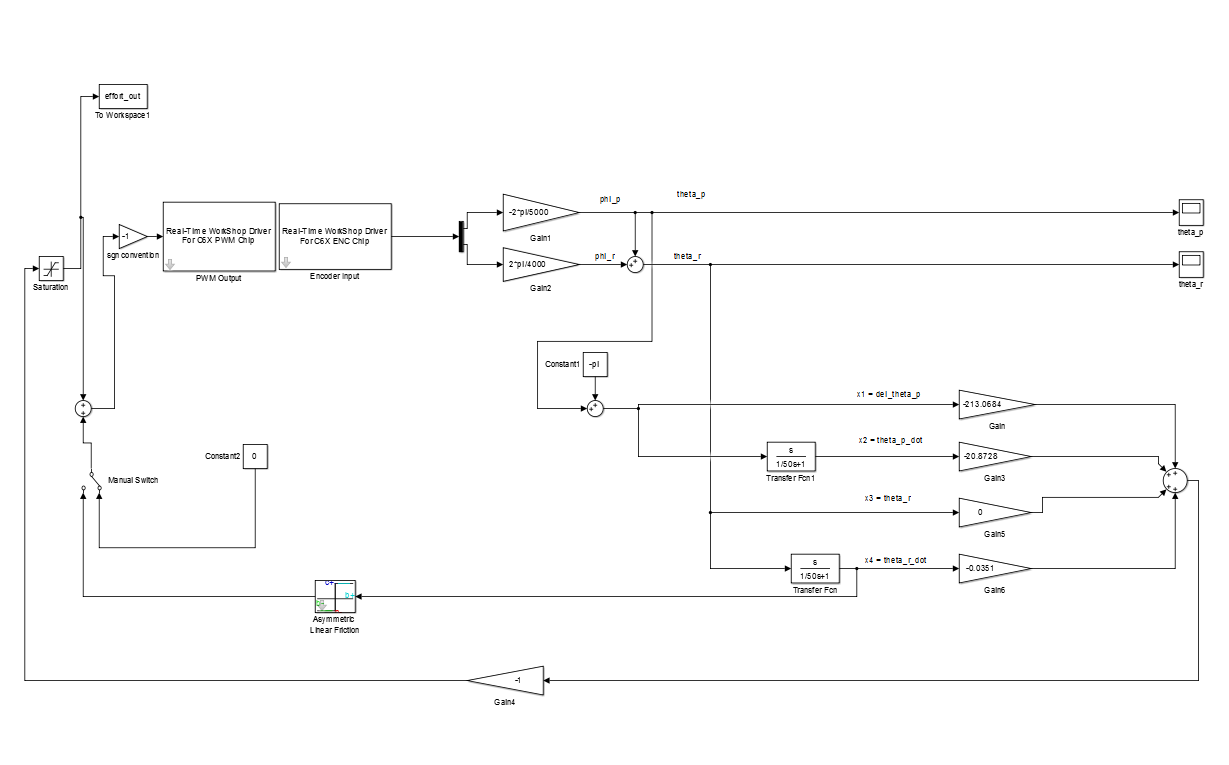
\includegraphics[scale = 0.4]{three_state.PNG}
\end{figure}

\subsection{Mathematical Proof}
We want to prove though that this does indeed create a stable system.

Our system can be described as follows:
$\boldsymbol{\dot x = Ax+B}u$

$$
\begin{bmatrix}
\delta\dot\theta_p\\
\ddot\theta_p\\
\delta\dot\theta_r\\
\ddot\theta_r
\end{bmatrix}
=
\begin{bmatrix}
0 & 1 & 0 & 0\\
a & 0 & 0 & 0\\
0 & 0 & 0 & 1\\
0 & 0 & 0 & 0
\end{bmatrix}
\begin{bmatrix}
\delta\theta_p\\
\dot\theta_p\\
\delta\theta_r\\
\dot\theta_r
\end{bmatrix}
+
\begin{bmatrix}
0\\
-b_p\\
0\\
b_r
\end{bmatrix}
u$$

We designed the pole locations of the closed-loop system to be at $(3^\frac{1}{2}*5*j - 5)$,$(-3^\frac{1}{2}*5*i - 5)$,$5$,$0$ in order to satisfy the transient response requirements. All the poles are in the LHP and hence stable. Using place command, we get the controller to be [-213 -20.8 0 -0.0351].Rewriting the system equation to be:
$\boldsymbol{\dot x = Ax+B}u$

$$
\begin{bmatrix}
\delta\dot\theta_p\\
\ddot\theta_p\\
\delta\dot\theta_r\\
\ddot\theta_r
\end{bmatrix}
=
\begin{bmatrix}
0 & 1 & 0 & 0\\
-150 & -21.8 & 0 & -0.0367\\
0 & 0 & 0 & 1\\
41597 & 4075 & 0 & 6.8476
\end{bmatrix}
\begin{bmatrix}
\delta\theta_p\\
\dot\theta_p\\
\delta\theta_r\\
\dot\theta_r
\end{bmatrix}
$$

At steady state, the $\dot x$ should be zero. Setting $\dot x$ to 0 and using Matlab, we computed the solution of the equation to be $[0 0 0 0]^T$. This means that  $\delta\theta_p=0$ $\dot\theta_p=0$  $\dot\theta_r=0$  are the only stable equilibrium for the equation.  This means that the system will stablize to the inverted position at steady state.

\subsection{Robustness Comparisons}
The following table shows our simulated robustness results. One can see that our three state feedback was able to withstand the largest pulse and disturbance forces and still stay stable.\\
\begin{tabular}{|c|c|c|c|}
\hline
 & Two-state Feedback & Three-state Feedback & Observer\\ \hline
 & $\delta\theta_p$  $\delta\theta_r$ & $\delta\theta_p$  $\delta\theta_r$ & $\delta\theta_p$  $\delta\theta_r$\\ \hline
Max IC deviations & 0.12  1.1 & 0.12  1 & 0.12  0.99\\ \hline
Max pulse & 7.5 & 8.1 & 7\\ \hline
Max disturbance & 5 & 7.4 & 6.3\\
\hline
\end{tabular}
\subsection{System Behavior}
With the controller, the system will be stabilized at the equilibrium point $\theta_p= \pi$. From the Windows Target implementation, we see that the system is able to adjust and stabilize to the top position with small initial deviations. It could also reject gentle tap which represent a pulse disturbance as well as the constant disturbance. As such, the system is stabilized by the controller we designed at the top position and it has certain degree of robustness to resist disturbances. We also took note that frictional forces here benefit us and damps out distrubances.
% This file is part of the multi-tex ECE 486 Final Project Report 
% file name: 4-full-state-feedback-control-decoupled-observer.tex

% YOU DO NOT COMPILE FROM THIS SINGLE FILE, read the following

% included files:
% (Makefile)
% Makefile -- run make Makefile (on Mac or Linux), it takes care of LaTeX compilation

% (*.PDF)
% report.pdf -- report file, print it out and submit it

% (*.TEX)
% report.tex -- main file, pdflatex this file (tested on Mac and Linux)
% 0-title-page.tex -- title page 
% 1-introduction.tex -- chapter 1 
% 2-mathematical-model.tex -- chapter 1 (lagrange equations of motion) and chapter 4 (linearisation)
% 3-full-state-feedback-control-friction-compensation.tex -- chapter 2 and chapter 4 (two state and three state feedback controller design) 
% 4-full-state-feedback-control-decoupled-observer.tex -- (this file) chapter 4 (controller design) and chapter 5 (observer design for estimated state)
% 5-conclusions.tex -- conclusion
% 6-extra-credit.tex -- (optional) add thsese pages if you have demoed chapter 6 and chapter 7

\section{Full State Feedback Control with Decoupled Observer}

\subsection{Theoretical Background}
The observer estimates the full states of the system given the output of the system. The observers are used when there are not enough sensors or when certain system states are not directly available. Hence we use the observer to estimate the full states of the system.  In our project, we use $\delta\theta_p$ and $\delta\theta_r$ to estimate the full states of the system.
For the RWP, the system matrix is:
$$
\begin{bmatrix}
0 & 1 & 0 & 0\\
a & 0 & 0 & 0\\
0 & 0 & 0 & 1\\
0 & 0 & 0 & 0
\end{bmatrix}
$$
The top right four values and the bottom left four values of the matrix are zero. It indicates that the pendulum and rotor subsystems are independent. This special form is called the block diagonal form. This special form allows us to decouple the matrix to two 2-by-2 matrices.
$$\dot x_{1,2} = 
\begin{bmatrix}
0 & 1 \\
a & 0
\end{bmatrix}
 x_{1,2}
+
\begin{bmatrix}
0 \\
-b_p
\end{bmatrix}
u, 
C_{1,2} = 
\begin{bmatrix}
1 & 0
\end{bmatrix}
$$
$$\dot x_{3,4} = 
\begin{bmatrix}
0 & 1\\
0 & 0
\end{bmatrix}
 x_{3,4}
+
\begin{bmatrix}
0 \\
b_r
\end{bmatrix}
u, 
C_{3,4} = 
\begin{bmatrix}
1 & 0
\end{bmatrix}
$$
The advantage of decoupling the matrix is that it allows the observer response to converge quickly. It also reduces the sensitivity of the system to state variations.\\
$$
L = 
\begin{bmatrix}
l_{11} & l_{12}\\
l_{21} & l_{22}\\
l_{31} & l_{32}\\
l_{41} & l_{42}
\end{bmatrix}
$$
Since the two decoupled systems are independent, the observer dynamics are determined by $l_{11}$ , $l_{21}$ , $l_{32}$, $l_{42}$. The other terms in the 4-state observer actually make the observer to be more sensitive to model errors and noise. By decoupling the observer, we could get rid of these terms and make the observer less sensitive and making the observer more robust.
\subsection{Derivation}
The error is given by:
$$e=x-\hat{x}$$
Differentiating the equation we get:
$$\dot e=\dot x- \hat{\dot x}$$
$$\dot e=Ax+Bu-A\hat{x}-Bu-L(y-C\hat{x})$$
$$\dot e=Ax-A\hat{x}-L(Cx-C\hat{x})$$
$$\dot e=Ax-LC\hat{x}-(A\hat{x}-LC\hat{x})$$
$$\dot e=(A-LC)(x-\hat{x})$$
This is equivalent to:
$$\dot e=(A-LC)e$$
We set the poles of our observer to be [-100 -99 -98 -96] and our L matrix is:
$$
L = 
\begin{bmatrix}
196 & 1.61\\
-9637 & -159\\
-1.37 & -196\\
-135 & -9667
\end{bmatrix}
$$
At steady state $\dot e$should be equal to zero. Our A-LC matrix is:
$$
A-LC = 
\begin{bmatrix}
196 & 1 & 1.61 & 0\\
-9637 & 0 & -159 & 0\\
-1.37 & 0 & -196 & 1\\
-135 & 0 & -9667 & 0
\end{bmatrix}
$$

The poles are at: [-100 -99 -98 -96] which are all stable LHP poles.

By using Matlab, we find that the unique solution to the above matrix equation is:
$$e=
\begin{bmatrix}
0\\
0\\
0\\
0
\end{bmatrix}
$$
As such, we can see that the $e = [0 0 0 0]^T$ is the only sable equilibrium for this equation. This means that the observer states will converge to the real states over time.

\begin{figure}
  \caption{Our control block diagram of our observer feedback with friction compensation}
  \centering
    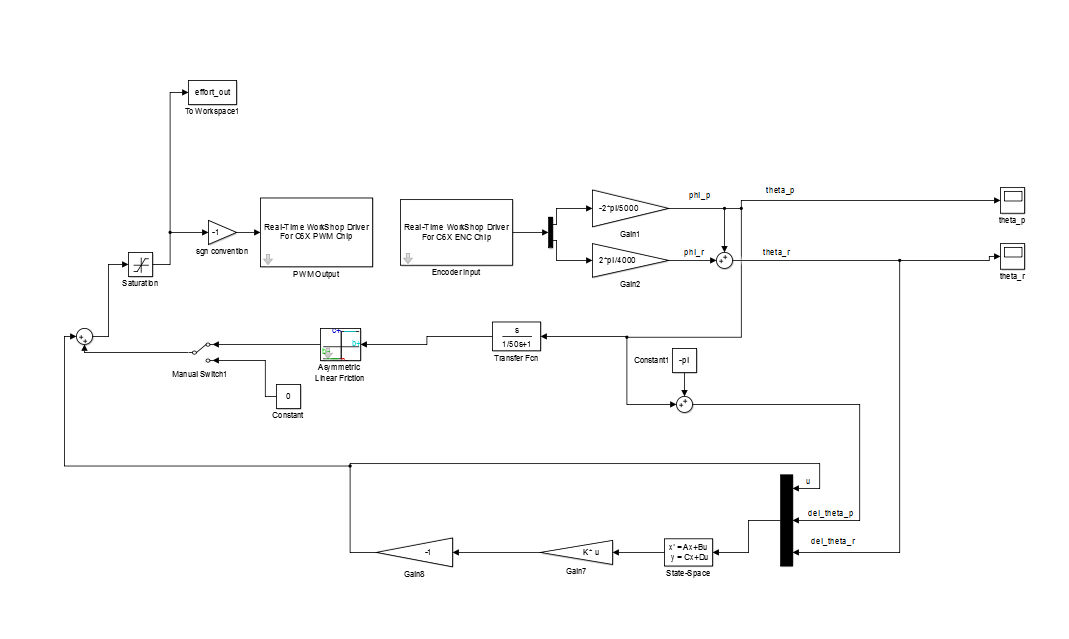
\includegraphics[scale = 0.4]{observe.PNG}
\end{figure}

\subsection{Robustness}
As shown below it's clear that our observer doesn't perform as well because it clearly can't do as well as direct access to the states.\\
\begin{tabular}{|c|c|c|c|}
\hline
 & Two-state Feedback & Three-state Feedback & Observer\\ \hline
 & $\delta\theta_p$  $\delta\theta_r$ & $\delta\theta_p$  $\delta\theta_r$ & $\delta\theta_p$  $\delta\theta_r$\\ \hline
Max IC deviations & 0.12  1.1 & 0.12  1 & 0.12  0.99\\ \hline
Max pulse & 7.5 & 8.1 & 7\\ \hline
Max disturbance & 5 & 7.4 & 6.3\\
\hline
\end{tabular}
\subsection{System Behavior}
The observer approach could also stabilize the system at the equilibrium point. The observer design has higher sensitivity than the full-state design meaning that the observer design could only reject smaller pulse, constant disturbances than the full-state controller. This means that the observer feedback controller is not as robust as the full-state feedback controller. The observer design has higher sensitivity since it could only estimate the approximate values of the states of the system.
% This file is part of the multi-tex ECE 486 Final Project Report 
% file name: 5-conclusions.tex

% YOU DO NOT COMPILE FROM THIS SINGLE FILE, read the following

% included files:
% (Makefile)
% Makefile -- run make Makefile (on Mac or Linux), it takes care of LaTeX compilation

% (*.PDF)
% report.pdf -- report file, print it out and submit it

% (*.TEX)
% report.tex -- main file, pdflatex this file (tested on Mac and Linux)
% 0-title-page.tex -- title page 
% 1-introduction.tex -- chapter 1 
% 2-mathematical-model.tex -- chapter 1 (lagrange equations of motion) and chapter 4 (linearisation)
% 3-full-state-feedback-control-friction-compensation.tex -- chapter 2 and chapter 4 (two state and three state feedback controller design) 
% 4-full-state-feedback-control-decoupled-observer.tex -- chapter 4 (controller design) and chapter 5 (observer design for estimated state)
% 5-conclusions.tex -- (this file) conclusion
% 6-extra-credit.tex -- (optional) add thsese pages if you have demoed chapter 6 and chapter 7

\section{Conclusions}
Both controllers have advantages and disadvantages over the other. In terms of robustness, the full-state feedback controller performs better over the observer design. This is shown by the robustness comparison table. The full-state feedback design can handle larger pulse and constant disturbance than the observer design. The full-state design has access to all the states of the system while the observer design could only estimate the states, hence, the full-state design will have higher precision to the states of the system and hence be more robust as compared to the observer design.
% This file is part of the multi-tex ECE 486 Final Project Report 
% file name: 6-extra-credit.tex

% YOU DO NOT COMPILE FROM THIS SINGLE FILE, read the following

% included files:
% (Makefile)
% Makefile -- run make Makefile (on Mac or Linux), it takes care of LaTeX compilation

% (*.PDF)
% report.pdf -- report file, print it out and submit it

% (*.TEX)
% report.tex -- main file, pdflatex this file (tested on Mac and Linux)
% 0-title-page.tex -- title page 
% 1-introduction.tex -- chapter 1 
% 2-mathematical-model.tex -- chapter 1 (lagrange equations of motion) and chapter 4 (linearisation)
% 3-full-state-feedback-control-friction-compensation.tex -- chapter 2 and chapter 4 (two state and three state feedback controller design) 
% 4-full-state-feedback-control-decoupled-observer.tex -- chapter 4 (controller design) and chapter 5 (observer design for estimated state)
% 5-conclusions.tex -- conclusion
% 6-extra-credit.tex -- (this file) (optional) add thsese pages if you have demoed chapter 6 and chapter 7

\section{Extra Credit: Up and Down Stabilizing Control}
Section 6 is about stabilizing the RWP at two different equilibrium positions. One is at the top position which is what we implemented in the previous part. The other one equilibrium point is the point at the bottom. 
Since the two equilibrium points are different, we need two sets of controllers to handle each point separately. We first linearized the system at the point $\theta_p=0$. Using the same set of pole locations. We get the controller to be [-73.5, -7.79, 0, 0.0351]. 
To switch between the two controllers, we used two conditional switches in our design to switch between the two controllers. We used the function $\cos(⁡\theta_p)$ to determine whether the pendulum is at the bottom or top positions and then switch to the corresponding controller. In addition, we also supplied two different offsets to get $\delta\theta_p$ at the two different positions. The offset is $\pi$ at the top position and is 0 at the bottom position.

\begin{figure}
  \caption{Our control block diagram of our Up-Down Control}
  \centering
    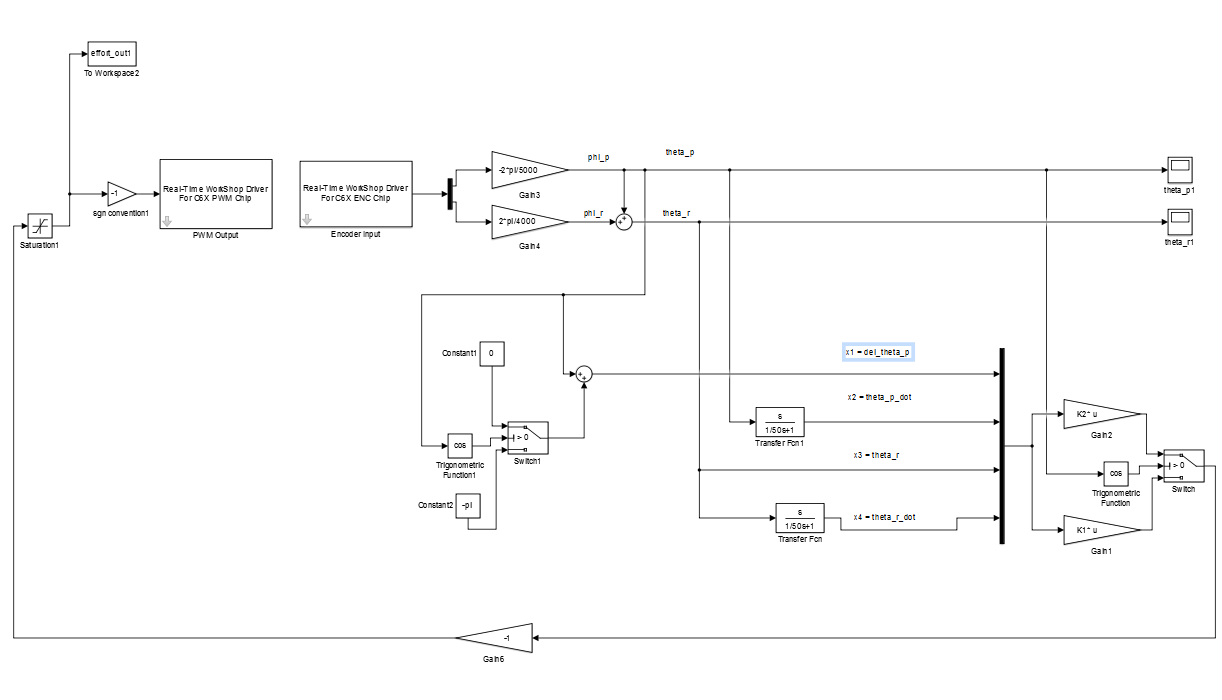
\includegraphics[scale = 0.4]{updown.PNG}
\end{figure}

\section{Extra Credit: Swing-Up Control}
We implemented section 7 by supplying forces along the direction of the swing of the pendulum to make it swing up to the equilibrium position.
In this section, we used 5 conditional switches to implement the swing-up controllers. The first conditional switch is used to switch between two situations where the pendulum is at left or right to the mount. For each situation, we have two switches. The conditions to the two switches are the angular velocities of the pendulum. When the angular velocities start to change sign, i.e. the pendulum has reached its maximum height in one swing, we supply a constant force along the direction to increase its kinetic energy. The other switch is used to handle the situation of overshoot. When the pendulum is swinging too fast – in the case we manually pushed the pendulum down from the top positions – the switch will switch to supplying no force so that the pendulum will be slowed and then return to the equilibrium position. With some trials, we determined that the best force to supply to our pendulum is 5 which will ensure a rather smooth swing to the top position.

\begin{figure}
  \caption{Our control block diagram of our Swing-Up Control}
  \centering
    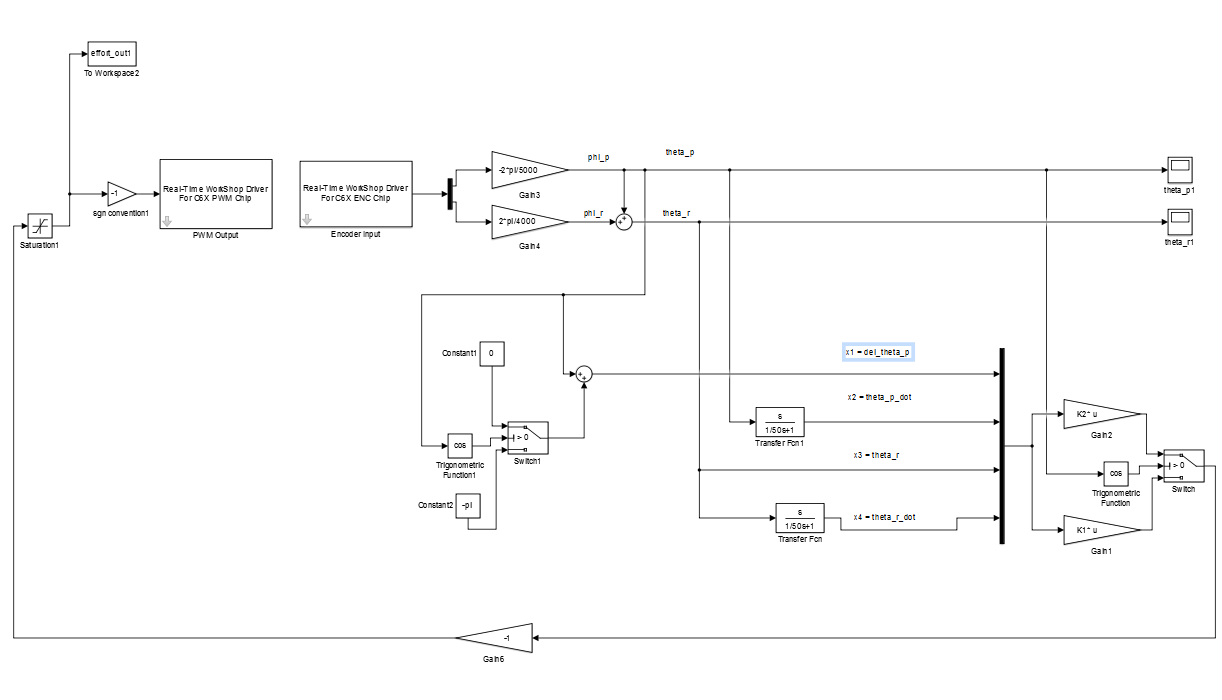
\includegraphics[scale = 0.4]{updown.PNG}
\end{figure}

% references
%\bibliographystyleltex{unsrt}
%\bibliographyltex{bib}

%\renewcommand{\refname}{Bibliography}

% bibliography
%\bibliographystyle{plain}
%\bibliography{bib}

\end{document}





%%% Local Variables:
%%% mode: latex
%%% TeX-master: t
%%% End:
